\documentclass{article}
\usepackage[a4paper, total={6in, 8in}]{geometry}
\begin{document}



\section{Memory}

\begin{itemize}
    \item Cycle Time - Minimum time between unrelated accesses to memory
    \item Access Time -  Time between a read is requested and when a word arrives.
\end{itemize}


\subsection{SRAM}

Static Random Access Memory. Typically used in caches, but not main memory. No refresh needed due to static nature. Access time is very close to cycle time. Typically uses 6 transistors/bit to avoid data disruption. Low power consumption at idle. 

\subsection{DRAM}

Dynamic Random Access Memory.

The dynamic nature of circuits in DRAM  requires data to be written back after being read. This is what causes disparity between access time and cycle time. Single transistor used per bit. 

Due to electronic properties, reads from a DRAM row destroy information. This means that it must be written back from the ??row buffer??. Bits must also be refreshed to prevent leakage (this usually happens in ms)

\subsubsecton{SDRAM}

There was an asynchronous interface for doing multiple column accesses on a single row that required an async interface. SDRAM adds a clock signal so repeated transfers would not bear overhead. Multiple banks added (with overlapping) allowing multiple row buffers on one chip. Requests being sent to a new bank are subject to additional delays due to the need to 'open' the bank. 


\subsubsecton{DDR DRAM}

Double data rate. Can transfer data on rising and falling edges of clock.

\subsubsection{GDDR DRAM}

Graphics DDR DRAM. Sacrafices latency/speed for increased bandwidth. Good for graphics-intensive tasks. GDDR5 was based on DDR3 specifications.

\subsection{Flash Memory}

A type of EEPROM (Electronically erasable programmable read only memory). Read only but can be erased. This is the technology used in most SSDs. Reads are sequential and read an entire $512$ to $4096$ byte page. Data must be erased before being written over. Much slower than DRAM. Keeps data even when power is lost.

\subsection{Phase-Change Memory}

Research toy. Uses heating element to change conductivity element of substrate. 

\subsection{Enhancing Dependability in memory systems}

Memory systems have 2 kinds of faults: Hard Errors (occur during fabrication or circuit cahnge during operation such as failure of a cell, mitigated by adding spare rows to tolerate failure) and Soft Errors/Transient Faults/Dynamic Errors (occur during normal operation whenever changes happen in a cell's contents i.e. bitflip). Errors can be detected with parity bits and fixed by error correcting codes. 

\section{Cache Improvement Strategies}
\begin{itemize}
    \item Smaller and less-associative high level caches
    \item Add banks to cache so that access does not activate whole cache
    \item Keep extra bits in cache to predict the next block access in cache (similar to branch prediction)
    \item Pipeline access and multibanked caches can increase bandwidth
    \item Non blocking caches allow for out-of-order execution computers to not stall waiting for cache 
    \item On a miss, request the missed word first so processor isn't waiting as long (Critical word first) OR On a miss, fetch in normal order and when missed word is rec'd send to processor (Early restart) 
    \item Compiler optimizations can fix things to have better spatial/temporal locality 
    \item Prefetching: predict next accesses and fetch them into cache before requested 
    \item Compiler Controlled prefetching: compiler inserts prefetch instructions 
    \item Have an L4 cache with high bandwidth memory technology
\end{itemize}

\section {Virtual Memory}
Basically what was learned in OS.

\sectiom{Cache Misses}

Compulsory - first time data is read
Conflict -  previously conflicted
Capacity - not enough room

\section{Cache Coherency Protocols}

Used to synchronize the data across caches.

\subsection{MSI}
Three states: Invalid, Modified, and Shared

\begin{itemize}
    \item Invalid - $v=0,d=0$ treated as not in cache
    \item Modified - $v=1,d=1$ we 'own' this data and can make writes 
    \item Shared - $v=1,d=0$ this data is up to date but we can't write to it as others have it
\end{itemize}

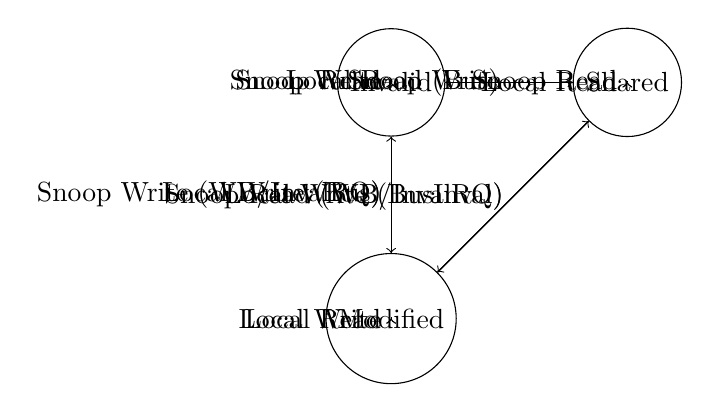
\begin{tikzpicture}
    \node[shape=circle,draw=black] (Invalid) at (0,3) {Invalid};
    \node[shape=circle,draw=black] (Modified) at (0,0) {Modified};
    \node[shape=circle,draw=black] (Shared) at (3,3) {Shared};

    \path [->] (Invalid) edge node[left] {Local Write (Bus)} (Modified);
    \path [->] (Invalid) edge node[left] {Local Read  (Bus)} (Shared);
    \path [->] (Invalid) edge node[left] {Snoop Read} (Invalid);
    \path [->] (Invalid) edge node[left] {Snoop Write} (Invalid);
    
    \path [->] (Modified) edge node[left] {Local Write} (Modified);
    \path [->] (Modified) edge node[left] {Local Read} (Modified);
    \path [->] (Modified) edge node[left] {Snoop Read (WB/InvalRQ)} (Shared);
    \path [->] (Modified) edge node[left] {Snoop Write (WB/InvalRQ)} (Invalid);
    
    \path [->] (Shared) edge node[left] {Local Write (BusInval)} (Modified);
    \path [->] (Shared) edge node[left] {Local Read} (Shared);
    \path [->] (Shared) edge node[left] {Snoop Read} (Shared);
    \path [->] (Shared) edge node[left] {Snoop Write} (Invalid);
\end{tikzpicture}

\subsection{MESI}

Four states: Modified, Exclusive, Shared, and Invalid. This extension reduces amount of communication on bus.
Best for multiprogramming workloads where cores are running different processes and generally don't share data.

\begin{itemize}
    \item Exclusive - Bock is present in $1$ class and is clean. Can write without invalidating
\end{itemize}

% DOUBLE CHECK ME!
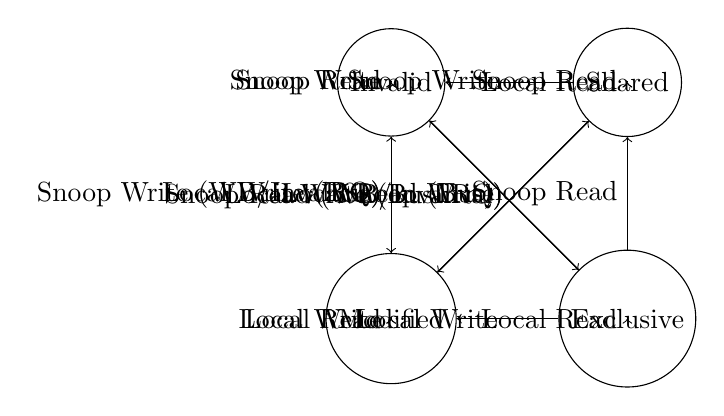
\begin{tikzpicture}
    \node[shape=circle,draw=black] (Invalid) at (0,3) {Invalid};
    \node[shape=circle,draw=black] (Modified) at (0,0) {Modified};
    \node[shape=circle,draw=black] (Shared) at (3,3) {Shared};
    \node[shape=circle,draw=black] (Exclusive) at (3,0) {Exclusive};

    \path [->] (Invalid) edge node[left] {Local Write (Bus)} (Modified);
    \path [->] (Invalid) edge node[left] {Local Read  (Bus)} (Exclusive);
    \path [->] (Invalid) edge node[left] {Snoop Read} (Invalid);
    \path [->] (Invalid) edge node[left] {Snoop Write} (Invalid);
    
    \path [->] (Modified) edge node[left] {Local Write} (Modified);
    \path [->] (Modified) edge node[left] {Local Read} (Modified);
    \path [->] (Modified) edge node[left] {Snoop Read (WB/InvalRQ)} (Shared);
    \path [->] (Modified) edge node[left] {Snoop Write (WB/InvalRQ)} (Invalid);
    
    \path [->] (Shared) edge node[left] {Local Write (BusInval)} (Modified);
    \path [->] (Shared) edge node[left] {Local Read} (Shared);
    \path [->] (Shared) edge node[left] {Snoop Read} (Shared);
    \path [->] (Shared) edge node[left] {Snoop Write} (Invalid);
    
    \path [->] (Exclusive) edge node[left] {Local Read} (Exclusive);
    \path [->] (Exclusive) edge node[left] {Local Write} (Modified);
    \path [->] (Exclusive) edge node[left] {Snoop Read} (Shared);
    \path [->] (Exclusive) edge node[left] {Snoop Write} (Invalid);
\end{tikzpicture}

\subsection{MOESI}

Five states: Modified, Owned, Exclusive, Shared, and Invalid. Reduces the number of 
writebacks/reads from main memory when data is in another cache. 

\begin{itemize}
    \item Owned - This cache has a copy of this block, but other caches might have a shared copy of block. Memory may not be synced. Only this cache replies to bus reads.
\end{itemize}

% DOUBLE CHECK ME!
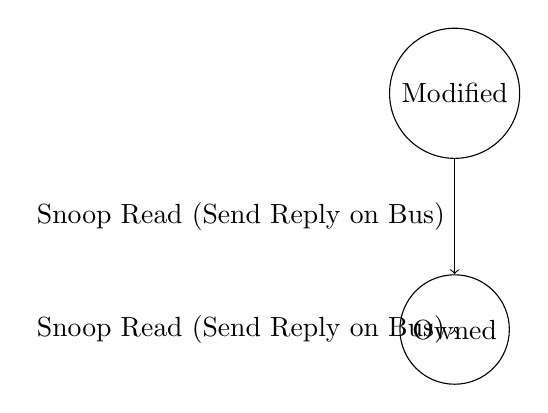
\begin{tikzpicture}
    \node[shape=circle,draw=black] (Owned) at (0,0) {Owned};
    \node[shape=circle,draw=black] (Modified) at (0,3) {Modified};
    \path [->] (Owned) edge node[left] {Snoop Read (Send Reply on Bus)} (Owned);
    \path [->] (Modified) edge node[left] {Snoop Read (Send Reply on Bus)} (Owned);
\end{tikzpicture}

\subsection{Distributed Shared Memory}

Non-shared memory treats each core as it's own computer. Each core can only access a set of memory.
DSM allows for each core to access different parts of memory. Non-shared generally uses memory passing, 
design choices made to facillitate NSM can lead to better performance. 

\subsection{Directory based}

Instead of sending everything over a bus, each processor has a directory controller than manages
a part of memory. P2P communication between directory controllers. 

\section{Pipelining}

\subsection{Branch prediction

Static branch prediction looks at previous run results (usually bimodally distributed) and 
always takes the more probable case. Dynamic ones use a bit (or more) to track if the current 
pc has been taken recently and follow that pattern (ls bits of pc are indexed into buffer 
tracking this).

\subsection{Hazards}

Hazards are things that can mess up pipelining
Some reads can be hazardous due to DMA.

\begin{itemize}
    \item RAW - Read after write. Most common. 
    \item WAR - Write after read. Only a problem in OOO
    \item WAW - Write after write. Only a problem in OOO
    \item Branching - More expensive than data. These are hazards that may or may not change PC based on input. 
\end{itemize}

Methods to combat Hazards

\begin{itemize}
    \item Forwarding - Forward result from execute/memory and memory/writeback and feed back to ALU for inputs
    \item Stalling - Slow 
    \item 
\end{itemize}

\end{document}
